\documentclass[a4paper]{article}
\author{Rendy Putra Pratama - 140310230037}
\title{Tugas Sistem Persamaan Linear Fisis}
\date{}
\usepackage[left=3.00cm, right=2.00cm, bottom=2.00cm, top=2.00cm]{geometry}
\usepackage{booktabs}
\usepackage{graphicx}
\usepackage{amsmath}
\usepackage{hyperref}
\usepackage[nice]{nicefrac}
\usepackage{xfrac}
\usepackage{listings}
\usepackage{xcolor}
\definecolor{codegreen}{rgb}{0,0.6,0}
\definecolor{codegray}{rgb}{0.5,0.5,0.5}
\definecolor{codepurple}{rgb}{0.58,0,0.82}
\definecolor{backcolour}{rgb}{0.95,0.95,0.92}

%Code listing style named "mystyle"
\lstdefinestyle{mystyle}{
  backgroundcolor=\color{backcolour},   commentstyle=\color{codegreen},
  keywordstyle=\color{magenta},
  numberstyle=\tiny\color{codegray},
  stringstyle=\color{codepurple},
  basicstyle=\ttfamily\footnotesize,
  breakatwhitespace=false,         
  breaklines=true,                 
  captionpos=b,                    
  keepspaces=true,                 
  numbers=left,                    
  numbersep=5pt,                  
  showspaces=false,                
  showstringspaces=false,
  showtabs=false,                  
  tabsize=2
}

%"mystyle" code listing set
\lstset{style=mystyle}

\begin{document}
\maketitle
\section{Sistem Pegas}
Sistem
yang ditunjukkan pada gambar terdiri dari \textbf{n} buah pegas linier yang menopang n
buah benda bermassa \textbf{m}. Konstanta pegas disimbolkan dengan \textbf{k} berat benda adalah
\textbf{w} dan \textbf{x} adalah perpindahan benda diukur dari posisi pegas saat tidak terdeformasi.
Persamaan perpindahan diperoleh dengan menuliskan persamaan keseimbangan
setiap benda dan mengganti $\vec{F}$ dengan gaya pegas diperoleh persamaan sebagai
berikut $:$

\begin{align*}
(k_1 + k_2)\cdot x_1 - k_2 \cdot x_2 &= w_1 \\
-k_i\cdot x_{i-1} + (k_i+k_{i+1})x_i - k_{i+1}\cdot x_{i+1} &= w_i\\
i = 1,2,3,..., n-1\\
-k_n\cdot x_{n-1}+k_n \cdot x_n &= w_n
\end{align*}
Tuliskan
kode python untuk mendapatkan solusi dari sistem persamaan tersebut
dengan metode \textbf{Gauss Seidel} jika jumlah benda dan pegas 5 buah Diketahui nilai
konstanta pegas dan berat benda adalah sebagai berikut
\begin{align*}
k_1 = k_2 = k_3 &= 10\> \nicefrac{N}{mm} \\
w_1 = w_3 = w_5 &= 100 \> N \\
k_4 = k_5 &= 5 \> \nicefrac{N}{mm} \\ 
w_2 = w_4 &= 50 \> N
\end{align*}
\begin{figure}[h!]
\centering
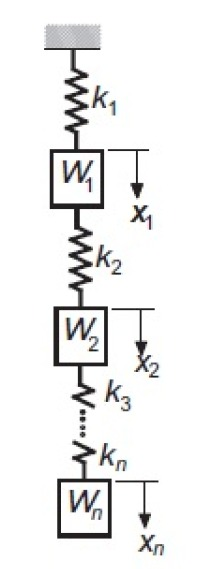
\includegraphics[width=2cm]{splpgs.jpeg}
\caption{Sistem Pegas}
\label{fig: Angular Position}
\end{figure}
\newpage
\subsection{Listing Program}
\lstinputlisting[language=Python, 
caption=Octave sample code
]{jacobi.py}
\subsection{Output Program}
\section{Rangkaian Listrik}

\end{document}